% -*-Latex-*-
% Debian config of GNU Alive
% Joachim Nilsson <joachim.nilsson@vmlinux.org>

% \documentclass[12pt, twocolumn, twoside]{article, report, letter, book}
\documentclass[12pt]{article}
% \usepackage{graphics}
% The following four rows are neccesary to be able to use Swedish.
\usepackage{a4wide}           % A4 dimensions
\usepackage[T1]{fontenc}      % Output of Latin 1 fonts.
\usepackage[english]{babel}   % Swedish t.o.c. and other stuff.
\usepackage[latin1]{inputenc} % Understand the ISO Latin 1 key set (eg. ������)
\usepackage{graphics}

\title{Debian Config of GNU Alive}
\author{Joachim Nilsson}

%\thanks{\copyright2005 Joachim Nilsson}
\begin{document}
\maketitle
%\begin{abstract}
%\end{abstract}

\section{Technical Information}

The Debian config file for GNU Alive was created when qadsl changed
name to GNU Alive.  The main reason for the creation was to facilitate
and smoothen the name change --- mainly to handle the transition of the
file \texttt{/etc/qadsl.conf} to \texttt{/etc/alive.conf}.

\begin{figure}
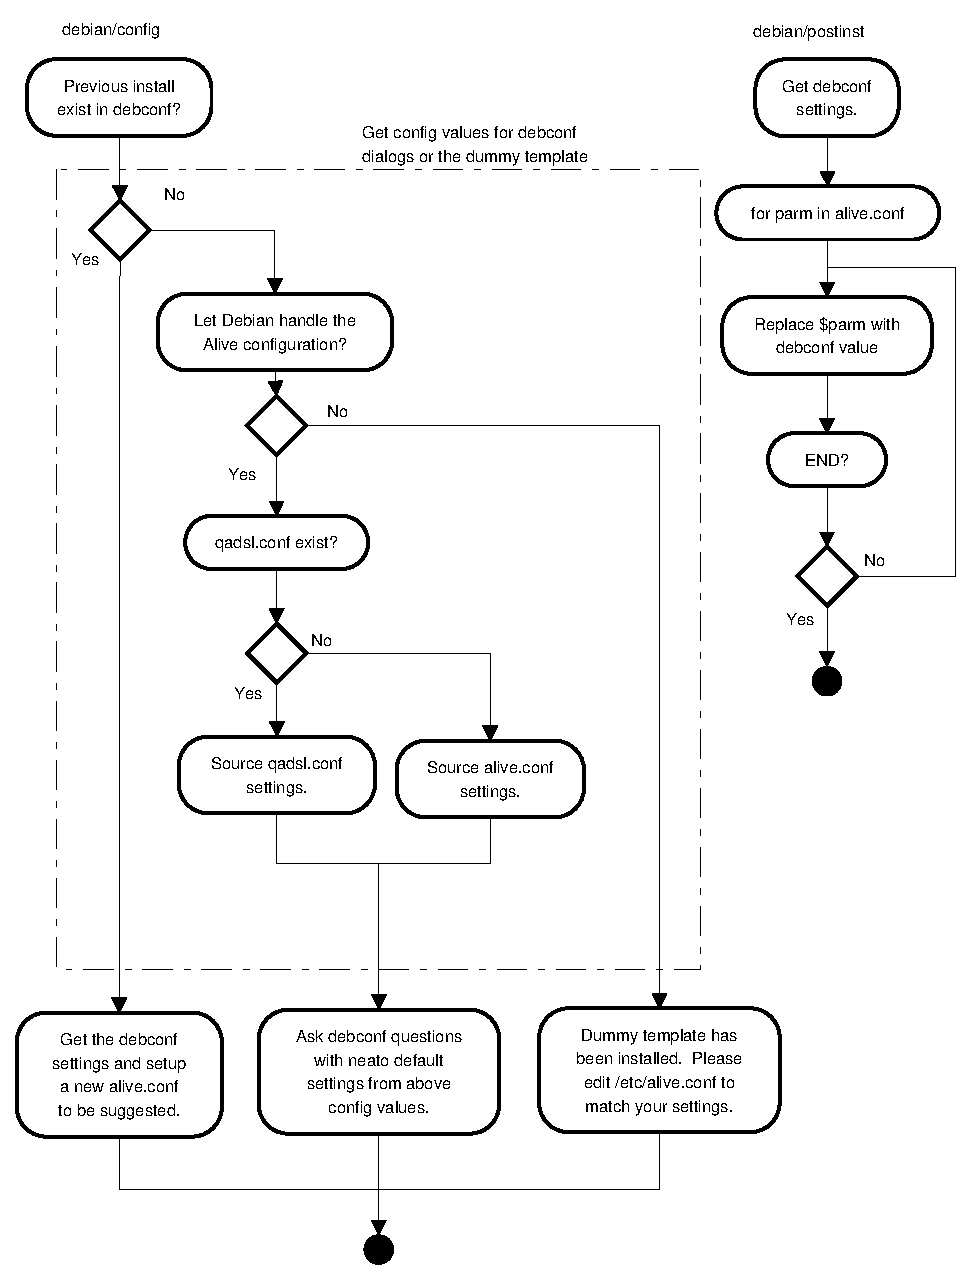
\includegraphics{config.eps}  % Don't forget to \usepackage{graphics} above.
\caption{Intended inner workings of the config script.}
\label{state-chart}  % Order *IS* dependent, caption first and THEN label!
\end{figure}


\section{Modus Operandi}
The first drafted intentions are shown in figure~\ref{state-chart}.
The actual operation, however, is as follows:

\begin{enumerate}
\item Check if there is anything registered for GNU Alive in debconf db.
  \begin{enumerate}
  \item If there is no trace of a previous config in the db then we
    pop the question: ``Do you want Debian to handle alive.conf?''
    \begin{enumerate}
    \item If the user selects ``No thanks'', then we do nothing more
      and leave it up to postinst do inform the user of the situation.
    \end{enumerate}
  \item Debian handles conf file: We first look for any old qadsl.conf
    \begin{enumerate}
    \item If qadsl.conf exists we source its settings as defaults for
      the debconf questions later. This can be somewhat tricky since
      the config language supports several aliases for settings.
    \end{enumerate}
  \item If no qadsl.conf we simply setup default values.
  \end{enumerate}
\item Ask debconf questions using the defaults set above, unless
  already quit.
\end{enumerate}

\end{document}
